%%%%%%%%%%%%%%%%%%%%%%%%%%%%%%%%%%%%%%%%%%%%%%%%%%%%%
% Author: Brian Detweiler
% Course: MATH 8756, Probability and Statistics II
%%%%%%%%%%%%%%%%%%%%%%%%%%%%%%%%%%%%%%%%%%%%%%%%%%%%%
% LaTeX Template for Project Report, Version 2.0
% (Abstracted from a Major Project Report at CSED, NIT Calicut but can be
% modified easily to use for other reports also.)
%
% Released under Creative Commons Attribution license (CC-BY)
% Info: http://creativecommons.org/licenses/by/3.0/
%
% Created by: Kartik Singhal
% BTech CSE Batch of 2009-13
% NIT Calicut
% Contact Info: kartiksinghal@gmail.com
%
% It is advisable to learn the basics of LaTeX before using this template.
% A good resource to start with is http://en.wikibooks.org/wiki/LaTeX/
%
% All template fields are marked with a pair of angular brackets e.g. <title here>
% except for the ones defining citation names in ref.tex.
%
% Empty space after chapter/section/subsection titles can be used to insert text.
%
% Just compile this file using pdflatex after making all required changes.

\documentclass[12pt,a4paper]{report}
\usepackage[pdftex]{graphicx} %for embedding images
\usepackage{url} %for proper url entries
\usepackage[bookmarks, colorlinks=false, pdfborder={0 0 0}, pdftitle={MATH 8756 Final Project}, pdfauthor={Brian Detweiler}, pdfsubject={Statistics and Scotch}, pdfkeywords={Statistics, Scotch}]{hyperref} 
\usepackage[toc,page]{appendix}
%for creating links in the pdf version and other additional pdf attributes, no effect on the printed document

%\usepackage[final]{pdfpages} %for embedding another pdf, remove if not required

%\usepackage[utf8]{inputenc}

%\usepackage{epigraph}
\usepackage{quotchap}
\usepackage[utf8]{inputenc}
\usepackage{amsmath}
\usepackage{amssymb}
\usepackage{color}
\usepackage{progressbar}
\usepackage{array}
\usepackage{tikz}
\usepackage{verbatim}
\usepackage{color,soul}
\usepackage{blkarray}
\usepackage[utf8]{inputenc}
\usepackage{amssymb}% http://ctan.org/pkg/amssymb
\usepackage{pifont}% http://ctan.org/pkg/pifont
\usepackage{listings}
\usepackage{mathtools}
\usepackage{csquotes}
\usepackage{algpseudocode}
\usepackage{wasysym}


%New colors defined below
\definecolor{codegreen}{rgb}{0,0.6,0}
\definecolor{codegray}{rgb}{0.5,0.5,0.5}
\definecolor{codepurple}{rgb}{0.58,0,0.82}
\definecolor{backcolour}{rgb}{0.95,0.95,0.92}

\DeclareMathOperator*{\as}{a.s.} 

%Code listing style named "mystyle"
\lstdefinestyle{mystyle}{
  backgroundcolor=\color{backcolour},   commentstyle=\color{codegreen},
  keywordstyle=\color{magenta},
  numberstyle=\tiny\color{codegray},
  stringstyle=\color{codepurple},
  basicstyle=\footnotesize,
  breakatwhitespace=false,         
  breaklines=true,                 
  captionpos=b,                    
  keepspaces=true,                 
  numbers=left,                    
  numbersep=5pt,                  
  showspaces=false,                
  showstringspaces=false,
  showtabs=false,                  
  tabsize=2
}

%"mystyle" code listing set
\lstset{style=mystyle}

%%%%%%%%%%%%%%%%%%%%%%%%%%%% EXAMPLE TABLE   %%%%%%%%%%%%%
%\begin{center}
%\begin{tabular}{ c c c }
% cell1 & cell2 & cell3 \\ 
% cell4 & cell5 & cell6 \\  
% cell7 & cell8 & cell9    
%\end{tabular}
%\end{center}



%%%%%%%%%%%%%%%%%%%%%%%%%%%% EXAMPLE PICTURE %%%%%%%%%%%%%
%\begin{figure}[htp]
%\centering
%\includegraphics[width=13cm]{Homework5_2.png}
%\caption{Bank Teller Queue}
%\label{fig:Queue}
%\end{figure}

%%%%%%%%%%%%%%%%%%%%%%%%%%%% EXAMPLE MATRIX %%%%%%%%%%%%%
%\begin{equation*}
%\begin{split}
%\begin{bmatrix}
%    x_{11}       & x_{12} & x_{13} & \dots & x_{1n} \\
%    x_{21}       & x_{22} & x_{23} & \dots & x_{2n} \\
%    \hdotsfor{5} \\
%    x_{d1}       & x_{d2} & x_{d3} & \dots & x_{dn}
%\end{bmatrix}
%&=
%\begin{bmatrix}
%    x_{11} & x_{12} & x_{13} & \dots  & x_{1n} \\
%    x_{21} & x_{22} & x_{23} & \dots  & x_{2n} \\
%    \vdots & \vdots & \vdots & \ddots & \vdots \\
%    x_{d1} & x_{d2} & x_{d3} & \dots  & x_{dn}
%\end{bmatrix}
%\end{split}
%\end{equation*}


%%%%%%%%%%%%%%%%%%%%%%%%%%% CODE EXAMPLE
%\begin{lstlisting}[language=R, caption=Evaluating Matrix H]
%\end{lstlisting}

\begin{document}

% Matrix variable boldface
\newcommand{\matr}[1]{\mathbf{#1}}
% I seem to typo this a lot, so we'll just alias it
\newcommand{\fraC}[2]{\frac{#1}{#2}}
% for repeating values
\newcommand*\repeating[1]{\overline{#1}}
\newcommand{\xmark}{\ding{55}}%

\makeatletter
\renewcommand*\env@matrix[1][*\c@MaxMatrixCols c]{%
  \hskip -\arraycolsep
  \let\@ifnextchar\new@ifnextchar
  \array{#1}}
\makeatother

\DeclarePairedDelimiter{\ceil}{\lceil}{\rceil}
\DeclarePairedDelimiter{\floor}{\lfloor}{\rfloor}


\renewcommand\bibname{References} %Renames "Bibliography" to "References" on ref page

%include other pages
\begin{titlepage}

Name: \textbf{Brian Detweiler}\\

\vspace{1in}

\textit{I have read the instructions and understand them. \textbf{The attached work is mine alone.}}

\vspace{1in}

Signed: 
\includegraphics[height=7\baselineskip]{sig} \par

\vspace{1in}

Date: Thursday, May 5th, 2016


\vfill

% Bottom of the page
\end{titlepage}
\begin{titlepage}

\begin{center}

\textup{\small {\bf MATH 8756 Final Project} \\ Report}\\[0.2in]

% Title
\Large \textbf {An Analysis of Scotch Whisky Prices}\\[0.5in]

%       \small \emph{Submitted in partial fulfillment of\\
%        the requirements for the award of the degree of}
%        \vspace{.2in}

%       {\bf Bachelor of Technology \\in\\ Computer Science and Engineering}\\[0.5in]

% Submitted by
\normalsize Submitted by \\
\begin{table}[h]
\centering
\begin{tabular}{lr}\hline \\
Brian Detweiler \\
\\ \hline
\end{tabular}
\end{table}

\vspace{.1in}
Thursday, May 5th, 2016
%{\textbf{<Guide's name here>}}\\[0.2in]

\vfill

% Bottom of the page


\end{center}

\end{titlepage}

\vspace{2in}
\begin{abstract}

In which we talk about scotch.

We will talk about

\begin{itemize}
    \item Sample Mean
    \item Variance
    \item Standard Deviation
    \item Boxplots 
    \item Point estimates for means
    \item Point estimates for variances
    \item Point estimates for std. devs
    \item Point estimates for proportions
    \item Bias
    \item Efficiency
    \item Consistency
    \item Sufficiency
    \item Confidence Intervals for means
    \item Confidence Intervals for difference of means
    \item Confidence Intervals for variances
    \item Confidence Intervals for ratio of two variances
    \item Confidence Intervals for proportions
    \item Confidence Intervals for difference between proportions
    \item Make confidence statements related to data
    \item Specify which statistic you use for computing the CI
    \item Specify under what assumption you work
    \item include formulas as necessary
    \item Find sample sizes that would be needed in order to decrease the max error to a desired value
    \item Testing hypotheses
    \item Test at least two hypotheses about means, differences of means (two means or ANOVA), variances, proportions (binomial or multinomial), independence (contingency table), goodness of fit
    \item State assumptions and draw conclusions in the context of the data
    \item Perform linear regression and / or normal correlation analysis
    \item Any other statistical aspects or tests
\end{itemize}

\end{abstract} 



\pagenumbering{roman} %numbering before main content starts
\tableofcontents
\listoffigures

\newpage
\pagenumbering{arabic} %reset numbering to normal for the main content


\begin{savequote}[45mm]
I love scotch. Scotchy, scotch, scotch. Here it goes down, down into my belly... 
\qauthor{Ron Burgundy, \textit{Anchorman}}
\end{savequote}

\chapter{Introduction}

It's easy to break a budget on alcohol, as many college students know. But it becomes exponentially easier with scotch whisky\footnote{Scotch whisky is spelled without the "e"} with the rarest of breeds fetching upwards of \$460,000.\cite{Macallan64} Even middling bottles can easily run over \$100, leaving many to wonder why anyone would spend their hard earned money on something that is sure to have the same net result as a \$10 bottle of cheap swill that can be mixed with cola.

Scotch drinkers tend to see this from a different angle. Scotch collecting and tasting can be a hobby (albeit a high-end one), and should not be equated with just drinking. Connoisseurs appreciate the arduous time spent producing the whisky, from the distillation to the aging and even the bottling and packaging. Scotch takes much longer to age than bourbon, due to the climate in Scotland, and produces a vastly different flavor profile. In the past, the typical age for scotch has been twelve years of rest in a barrel, but due to rising demands, many distilleries have been experimenting with younger batches. 

So called "no age statement" varieties have been rising in popularity, in part to meet market demand amid surging popularity and dwindling stock of longer aged whiskies. Scotch must be aged for three years by law, but for most scotches, desirability increases with the age. Is scotch \textit{better} with age? It's a subjective question, and it depends on the scotch, but suffice it to say, it is definitely \textit{different}. That topic is not discussed here. \textit{WhiskyAnalysis.com} does a detailed meta-critic analysis if you are interested in a statistical analysis of tasting notes. \cite{WhiskyAnalysis}

When it comes to the question of age and quality, perception may not match reality. Chivas Brothers (makers of \textit{The Glenlivet} and other whiskies) ran a survey in 2010 examining consumer perception of age pertaining to scotch. They found that the vast majority of consumers actively look for an age statement and see it as an indicator of quality. In fact, 94\% believe that the older a whisky is, the better it must be. \cite{Chivas} Of course, this is not necessarily true, but could this perception have an affect on price?

In this paper, we examine the prices of scotch and how it correlates to age. We will also look at various online retailers and compare them with each other. We also present an open source database of prices for over two thousand whiskies, which may serve as guide for making informed consumer decisions.

In an effort to keep this project manageable, several restrictions must be put in place to avoid scope creep. These restrictions include the following:

\begin{enumerate}
  \item Must be single malt scotch whisky
    \subitem Blends will not be considered
    \subitem Grain whiskies will not be considered
    \subitem Only whiskies from Scotland will be considered
  \item Only 750ml bottles available for retail purchase will be considered
    \subitem Gift sets will not be considered
    \subitem Bottles of smaller or larger sizes will not be considered
    \subitem UK standard sizes of 700ml were not considered
    \subitem Inventory is not considered (the bottle may be out of stock, so long as the price is available)
  \item Purchase minimums or maximums are not considered
  \item Shipping, handling, customs, or other fees are not considered \footnote{These would obviously play a big role in a purchase decision, but building a robust pricing schema is beyond the scope of this project}
\end{enumerate}



%\section{Background and Recent Research}
%\subsection{<any sub section here>}

%\subsection{Literature Survey}

%\subsubsection{<Sub-subsection title>}
%some text\cite{citation-1-name-here}, some more text

%\subsubsection{<Sub-subsection title>}
%even more text\footnote{<footnote here>}, and even more.

%\section{Motivation}
 %literature survey included in this
\chapter{Findings}

\section{Environment Setup}

\subsection{Gathering Data}

The most tedious part of a data scientist's job is data wrangling. It is a necessary evil, because often, interesting data does not exist as a clean, ready to use dataset. If we want the data, we capture and clean it.

To this end, the data we want is scotch, complete with name, distilleries, producers, ages, and prices.  There are some closed databases at \cite{WhiskyDotCom} and \cite{WhiskyStats}, and an interesting open database of tasting notes at \cite{WhiskyAnalysis}. Each of these probably have more information than what is gathered here, but this is produced as open source and allows and encourages others to build on this work.

The data wrangling method used here was quite unsophisticated, and not at all scalable. After a web search of online scotch retailers, twenty candidates were selected. We filtered each retailer's inventory by scotch whisky and scraped the results into text files. From there, it was mostly a manual cleaning effort, using Vim and regular expressions. Once the data had been organized into simple CSVs, a Python script was used to insert the data into a normalized SQLite database. 

After the data entry was complete, I meticulously went through and consolidated duplicate whiskies, distilleries, and producers by hand. The entire process took over a week to complete. In order to scale this up, automated methods would be necessary. Naive web scraping may not pass muster here, and more sophisticated methods, including Natural Language Processing may be necessary. For this project, the one-time manual effort was sufficient.

\subsection{Technical Notes}


All statistical analysis was done in a Jupyter Notebook with Python. Plots were created using Seaborn and Matplotlib. 

The CSVs were inserted into a SQLite database.

\begin{figure}[htb]
\centering
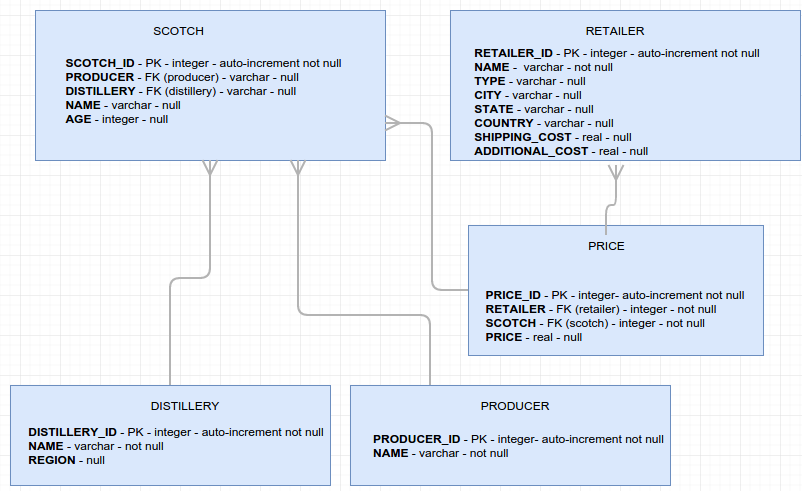
\includegraphics[scale=.5]{scotch_prices_schema}
\caption{Scotch Database Schema}
\label{fig:scotch_database_schema} 
\end{figure}

This entire project, complete with code, database, and \LaTeX  source can be found at \cite{GitHub}.

\subsection{Caveats}
One late-term regret was waiting until I had my full dataset to explore the data. This can introduce bias. A better approach would have been to load one retailer, explore the dataset, make hypotheses, load the rest, and see how my hypotheses hold up. \cite{StatisticsDoneWrong} However, this was a tricky dataset to obtain, so it comes inherent with some imperfections.



\section{Exploring the Data}



%%%%%%%%%%%%%%%%%%%%%%%%%%%%%%%%%%%%%%%%%%%%%%%%%
%%%%% Distribution of Age
%%%%%%%%%%%%%%%%%%%%%%%%%%%%%%%%%%%%%%%%%%%%%%%%%
\subsection{Distribution of Age}

Age of a whisky is the truncated amount of time in years that the youngest malt in the blend has spent in a barrel. This is a discrete random variable $X$ such that $X \in \{3, 4, \hdots, 75\}$. By law, scotch must be aged at least 3 years, or else it is called a \textit{spirit}. There is nothing saying that $X$ cannot exceed 75, however, as of this publication, the oldest known whisky is a \textit{Mortlach}, aged 75 years, produced by independent bottlers \textit{Gordon \& MachPhail}. Whisky evaporates as it is aged, so there is some upper bound - determined by physics - on how long it can remain in the barrel before it simply disappears. We will use the oldest known whisky as an upper bound on the population.

\begin{figure}[htb]
\centering
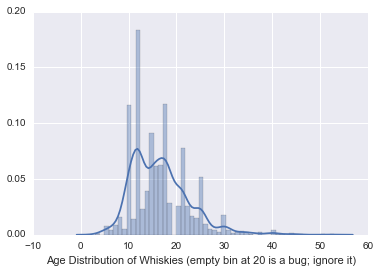
\includegraphics[scale=1]{age_distribution}
\caption{Age distribution of whiskies with age statements}
\label{fig:age_distribution} 
\end{figure}



\pagebreak


\begin{figure}[htb]
\centering
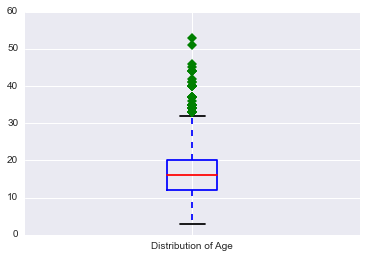
\includegraphics[scale=1]{boxplot_age} 
\caption{Age distribution of whiskies with age statements}
\label{fig:boxplot_age_distribution} 
\end{figure}


From the density plot, it quite clear that our distribution is non-normal. 

\pagebreak

From the boxplot, we can see that most ages fall between 12 and 21 years old, but there are a good amount of outliers that will skew the distribution.

It is interesting to note that twelve year old scotches dominate, accounting for over 17\% of the market. This is likely the "sweet spot" for whiskies with age statements, where distillers are able to minimize age and maximize quality and flavor. This is not true for all whiskies, of course, as flavor profiles differ for each whisky. However, in this quantitative analysis, we are interested generalizing and estimating the population. Randomness is inherent. 


\begin{center}
\begin{tabular}{ c c }
 Year & Frequency (percent)\\
 \hline
 \hline
    10 year olds & 10.889292196\\
    12 year olds & 17.0961887477\\
    15 year olds & 8.42105263158\\
    18 year olds & 11.0344827586\\
    21 year olds & 7.36842105263\\
    25 year olds & 5.00907441016\\
    30 year olds & 1.70598911071\\
\end{tabular}
\end{center}
\label{fig:most_common_ages}

We obtain the following statistics from our sample distribution of ages:

\begin{equation*}
\begin{split}
    n &= 2755 \\
    \overline{x} &=  15.6134946314 \\
    \widetilde{x} &= 16.0 \\
    s^2 &= 36.682608369 \\
    s &= 6.05551760361 \\
    \text{Skewness} &= 1.15380146462 \\
\end{split}
\end{equation*}

\pagebreak

%%%%%%%%%%%%%%%%%%%%%%%%%%%%%%%%%%%%%%%%%%%%%%%%%
%%%%% Distribution of Price
%%%%%%%%%%%%%%%%%%%%%%%%%%%%%%%%%%%%%%%%%%%%%%%%%
\subsection{Distribution of Price}

We could reasonably expect most of the prices to be in the more affordable region, as that's what sells best. After all, there are far more \textit{consumers} of whisky than collectors. There is a reason comparatively cheaper blends like Johnny Walker are the best selling scotches in the world. The economics dictate that the ROI will be stronger with quality products in the affordable region, and a few flashy showcase products to drum up envy and garner attention to the brand. We will treat price as a non-negative continuous random variable. 

\begin{figure}[htb]
\centering
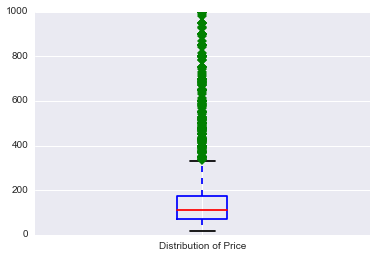
\includegraphics[scale=1]{boxplot_price} 
\caption{Price distribution of whiskies with age statements}
\label{fig:boxplot_price_distribution} 
\end{figure}

\begin{figure}[htb]
\centering
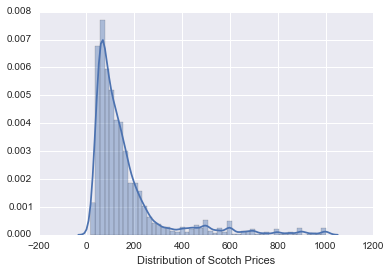
\includegraphics[scale=1]{price_distribution} 
\caption{Whisky price distribution}
\label{fig:price_distribution} 
\end{figure}

\pagebreak

\begin{figure}[htb]
\centering
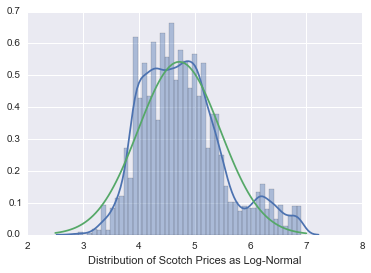
\includegraphics[scale=1]{price_distribution_log_normal}
\caption{Whisky price distribution as Log-Normal}
\label{fig:price_distribution_log_normal} 
\end{figure}

\pagebreak

We have the following statistics from the price distribution:

\begin{equation*}
\begin{split}
    n &= 2755 \\
    \overline{x} &=  119.165987296 \\
    \widetilde{x} &= 110.0 \\
    s^2 &= 26827.9806971 \\
    s &= 163.762763695 \\
    \text{Skewness} &= 2.72715134235 \\
\end{split}
\end{equation*}

Skewness is greater than 1, which indicates that this is heavily skewed to the right, so we cannot assume a normal distribution. Instead, what we have is closer to a \textbf{log-normal distribution}. This still has some skew to the right, but more closely resembles a bell curve. 


\pagebreak

The log-normal distribution is a transformation of the normal, written as $\ln{N(\mu, \sigma^2)}$. 

The log-normal has the following moments:

\begin{equation*}
\begin{split}
    \mu_{LN} &= e^{\mu + \frac{\sigma^2}{2}} \\
    \sigma_{LN}^2 &= (e^{\sigma^2} - 1)(e^{2\mu + \sigma^2}) \\
\end{split}
\end{equation*}

\begin{figure}[htb]
\centering
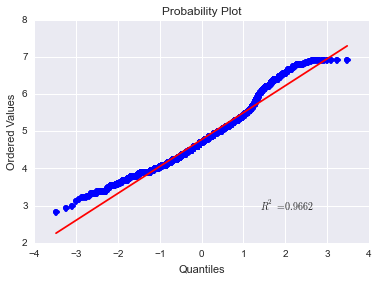
\includegraphics[scale=1]{price_pp_plot_log_normal} 
\caption{P-P Plot of Whisky Prices vs. Log-Normal}
\label{fig:price_pp_plot_log_normal} 
\end{figure}

Using a P-P plot, we can see how closely the log-normal follows a normal distribution. With an R-squared of 0.9662, it indicates a close goodness of fit. The bump in the tail at the high end is due to the bump in our pdf, where the prices have a slight increase in frequency in the \$600-\$700 range. No real world model matches a distribution 100\%, so we will accept this small imperfection.

\pagebreak


%%%%%%%%%%%%%%%%%%%%%%%%%%%%%%%%%%%%%%%%%%%%%%%%%
%%%%% Point Estimates
%%%%%%%%%%%%%%%%%%%%%%%%%%%%%%%%%%%%%%%%%%%%%%%%%
\subsection{Point Estimates}

Let $X_1 \hdots X_n$ be independent random variables having the log-normal distribution, $Y_i \sim \ln{N(\theta_1, \theta_2^2)}$. Then the transformation $Y_i = \ln{X_i}, i = 1, \hdots, n$ has the normal distribution, $N(\mu, \sigma^2)$ with mean $\mu$ and variance $\sigma^2$, such that

\begin{equation*}
\begin{split}
    \theta_1 &= e^{\mu + \frac{\sigma^2}{2}}\\
    \theta_2^2 &= e^{2 \mu + \sigma^2} \cdot (e^{\sigma^2} - 1)\\
\end{split}
\end{equation*}

Because of its relation to the normal, it is clear that $\overline{Y} = \frac{1}{n}\sum_{i = 1}^n \ln{X_i}$ and $S_Y^2 = \sum_{i = 1}^n (Y_i - \overline{Y})^2$. 

Using the result from Finney (1941), as mentioned by Shen (1998), we cat get unbiased MVUE estimators for $\theta_1$ and $\theta_2^2$ by first defining the infinite series, 

\begin{equation}
\begin{split}
    f(t) &= 1 + t + \frac{n - 1}{n + 1} \frac{t^2}{2!} + \frac{(n - 1)^2}{(n + 1)(n + 3)} \frac{t^3}{3!} + \hdots
\end{split}
\end{equation}

The adjusted unbiased MLEs are

\begin{equation}
\begin{split}
    \hat{\theta}_{MLE} &= e^{\overline{Y}} \cdot f\bigg(\frac{1}{2n} S_Y^2 \bigg)
\end{split}
\end{equation}

\begin{equation}
\begin{split}
    \hat{\theta_2^2}_{MLE} &= e^{\overline{2Y}} \cdot \bigg[f\bigg(\frac{2}{n} S_Y^2 \bigg) - f\bigg( \frac{n - 2}{n(n - 1)} S_Y^2\bigg) \bigg]
\end{split}
\end{equation}

Their variances are 

\begin{equation}
\begin{split}
    Var(\hat{\theta_1}_{MLE}) &= \frac{1}{n} \bigg(\sigma^2 + \frac{1}{2} \sigma^4 \bigg) e^{2 \mu + \sigma^2}
\end{split}
\end{equation}

\begin{equation}
\begin{split}
    Var(\hat{\theta_2^2}_{MLE}) &= \frac{2 \sigma^2}{n} e^{4 \mu + 2 \sigma^2} 
    \bigg[ 
        2 (e^{\sigma^2} - 1)^2 + \sigma^2 (2 e^{\sigma^2} - 1)^2
    \bigg]
\end{split}
\end{equation}

And since $Var(\hat{\theta_1}_{MLE}) \rightarrow 0$ and $Var(\hat{\theta_2^2}_{MLE}) \rightarrow 0$ as $n \rightarrow \infty$, the estimators are consistent.  \cite{Finney} \cite{Shen}


\pagebreak

\subsection{Confidence Intervals of Particular Scotch Prices}

As what I will call "research" for this project, I purchased a few bottles of scotch and took note of their prices. I wondered if I had gotten a fair deal on my purchases.

Among the acquisitions were an Auchentoshan Three Wood (no age statement) for \$63.00, a McClelland's Islay (also no age statement) for \$24.99, and a Laphroaig 10 Year Old, for \$50.00. 

We will compute 90\% confidence intervals to see if my purchases were within the expected mean. We will use the $t$-distribution, since our dataset only contains up to at most, 17 sample prices per scotch. \footnote{Due to some data cleaning issues, some scotch prices have been misplaced or incorrectly attributed. These three have been thoroughly inspected and cleaned, however.}

\begin{equation*}
\begin{split}
     \frac{\overline{X} - \mu}{\frac{S}{\sqrt{n}}} &\sim T(n - 1)
\end{split}
\end{equation*}

We have the following values


%%%%%%%%%%%%%%%%%%%%%%%%%%%% EXAMPLE TABLE   %%%%%%%%%%%%%
\begin{center}
\begin{tabular}{ c c c }
    Auchentoshan Three Wood & McClelland's Islay & Laphroaig 10 Year Old \\
    \hline
    \hline
    55.99 & 24.99 & 39.98 \\ 
    64.98 & 37.95 & 39.99 \\
    64.99 &       & 42.99 \\
    66.99 &       & 44.98 \\
    68.95 &       & 44.99 \\
    69.99 &       & 45.09 \\
    69.99 &       & 48.99 \\
    69.99 &       & 49.99 \\
    74.99 &       & 49.99 \\
    79.99 &       & 50.95 \\
    79.99 &       & 64.99 \\
\end{tabular}
\end{center}

Computing each separately, we find the mean and variance for the Auchentoshan to be
\begin{equation*}
\begin{split}
    n_{\text{Auchentoshan}} &= 11\\
    \overline{x}_{\text{Auchentoshan}} &= 69.71\\
    s_{\text{Auchentoshan}} &= 6.93\\
    \alpha &= 0.10\\
    t_{0.05, 10} &= 1.812\\
\end{split}
\end{equation*}

The 90\% confidence interval for the mean price of Auchentoshan Three Wood is 
\begin{equation*}
\begin{split}
    \bigg( \overline{X} - t_{\frac{\alpha}{2}, n - 1} \cdot \frac{S}{\sqrt{n}}
    &, 
    \overline{X} + t_{\frac{\alpha}{2}, n - 1} \cdot \frac{S}{\sqrt{n}} \bigg)\\
    \bigg( 69.71 - 1.812  \cdot \frac{6.93}{\sqrt{11}}
    &, 
    69.71 + 1.812  \cdot \frac{6.93}{\sqrt{11}} \bigg)\\
    (69.71 - 3.786 &, 69.71 + 3.786)\\
    (65.92 &, 73.50)\\
\end{split}
\end{equation*}

Since I paid \$63.00, I can feel confident that I got a below average price for my bottle, and I am likely to return to that particular vendor.

Calculating the mean and variance for the McClelland's, we get
\begin{equation*}
\begin{split}
    n_{\text{McLellands}} &= 2\\
    \overline{x}_{\text{McLellands}} &= 31.47\\
    s_{\text{McLellands}} &= 2.920 \\
    \alpha &= 0.10\\
    t_{0.05, 1} &= 6.314\\
\end{split}
\end{equation*}

The 90\% confidence interval for the mean price of McClelland's Islay is
\begin{equation*}
\begin{split}
    \bigg( \overline{X} - t_{\frac{\alpha}{2}, n - 1} \cdot \frac{S}{\sqrt{n}}
    &, 
    \overline{X} + t_{\frac{\alpha}{2}, n - 1} \cdot \frac{S}{\sqrt{n}} \bigg)\\
    \bigg( 31.47 - 6.314  \cdot \frac{2.920}{\sqrt{2}}
    &, 
    31.47 + 6.314  \cdot \frac{2.920}{\sqrt{2}} \bigg)\\
    (31.47 - 13.037 &, 31.47 + 13.037)\\
    (18.43 &, 44.50)\\
\end{split}
\end{equation*}

I paid \$25.00 for my bottle of McClelland's Islay (not a particularly good bottle either - a far-too-young Bowmore that could use a few more years in the barrel), and I can feel comfortable that I paid about average for my bottle, though more samples could tighten up that interval to be sure.

Finally, calculating the mean and variance for the Laphroaig, we find
\begin{equation*}
\begin{split}
    n_{\text{Laphroaig}} &= 11\\
    \overline{x}_{\text{Laphroaig}} &= 47.54\\
    s_{\text{Laphroaig}} &= 6.96\\
    \alpha &= 0.10\\
    t_{0.05, 10} &= 1.812\\
\end{split}
\end{equation*}

The 90\% confidence interval for the mean price of Laphroaig 10 Year Old is
\begin{equation*}
\begin{split}
    \bigg( \overline{X} - t_{\frac{\alpha}{2}, n - 1} \cdot \frac{S}{\sqrt{n}}
    &, 
    \overline{X} + t_{\frac{\alpha}{2}, n - 1} \cdot \frac{S}{\sqrt{n}} \bigg)\\
    \bigg( 47.54 - 1.812  \cdot \frac{6.96}{\sqrt{11}}
    &, 
    47.54 + 1.812  \cdot \frac{6.96}{\sqrt{11}} \bigg)\\
    (47.54 - 3.80 &, 47.54 + 3.80)\\
    (43.74 &, 51.34)\\
\end{split}
\end{equation*}

I paid \$50.00 for my bottle, which lands a little on the high side of the confidence interval, but still within it, so I can be confident I paid about average for it. And while it is nice to find bargains, we should be content knowing that we are not overpaying.

\pagebreak

%%%%%%%%%%%%%%%%%%%%%%%%%%%%%%%%%%%%%%%%%%%%%%%%%
%%%%% Regression and Correlation
%%%%%%%%%%%%%%%%%%%%%%%%%%%%%%%%%%%%%%%%%%%%%%%%%
\subsection{Regression and Correlation}

\begin{figure}[htb]
\centering
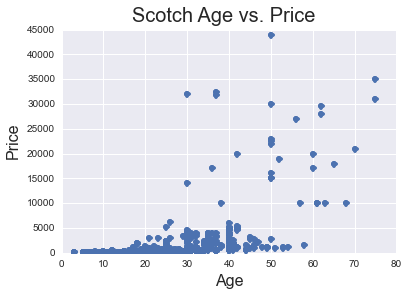
\includegraphics[scale=1]{age_vs_price1} 
\caption{Whiskies plotted by age vs. price showing a few significant outliers}
\label{fig:age_vs_price1} 
\end{figure}

\pagebreak

It is instantly clear that the majority of whiskies are priced below \$5000, but that there are some significant outliers. The majority of the outliers can be attributed to Macallan, which accounts for half of all whiskies over \$5000 in our samplings. The next closest distillery in priciness was Mortlach, which only accounted for 11\% of all whiskies over \$5000. Macallan is widely regarded as the "Rolls Royce" of whiskies and it shows in their prices.



\begin{figure}[htb]
\centering
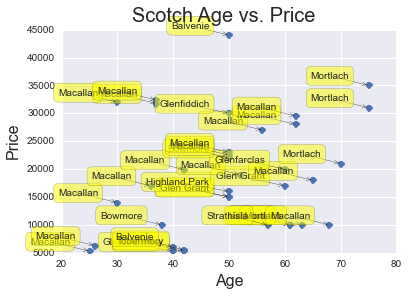
\includegraphics[scale=1]{age_vs_price_outliers} 
\caption{Age vs. Price - Outliers}
\label{fig:age_vs_price_outliers} 
\end{figure}

Since the more digestible range lies in the sub-\$5k category, let's zoom in on that.

\begin{figure}[htb]
\centering
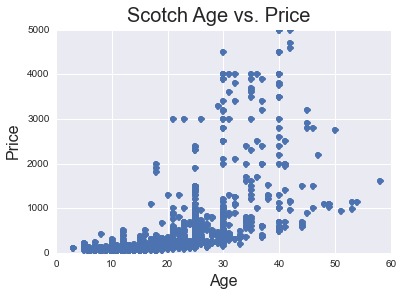
\includegraphics[scale=1]{age_vs_price2}
\caption{Whiskies plotted by age vs. price as a pattern starts to emerge}
\label{fig:age_vs_price2} 
\end{figure}

We can start to see a clear pattern here, though we are still very scattershot, particularly as the age progresses into the 20s and beyond. Notice, however, that there are some very old whiskies that are cheaper than some much younger whiskies. Just from this chart we can pick out an almost-60 year old whisky that is cheaper than a few late-teens whiskies. Right away, we can say that age does not imply price. It should start to become clear, that age is only one of many factors that are taken into account when pricing a whisky.

\pagebreak

We can see a very solid grouping below \$1000, so let's zoom in on that and add some linear regression.

\begin{figure}[htb]
\centering
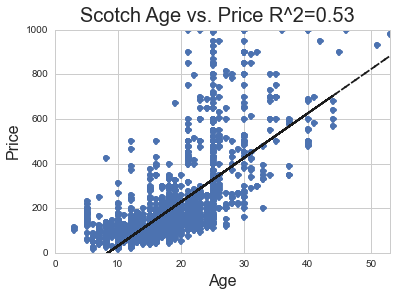
\includegraphics[scale=1]{age_vs_price3} 
\caption{Whiskies plotted by age vs. price with linear regression}
\label{fig:age_vs_price3} 
\end{figure}

The regression line is given by
\begin{equation*}
\begin{split}
    \hat{y} &= 19.7547958954 \cdot x  -165.573087176\\
\end{split}
\end{equation*}

I will once again caution against buying a whisky based solely on its age description, but this regression line would certainly be a good litmus test when purchasing a whisky that is not rare or collectible. If I'm buying a 21 year old whisky, I could expect my price to be around \$250. If I can find one for under \$200, it's worth considering. And yet, this chart shows there are a good number of sub-\$200 scotches in the 21 year old category. 


At this point, I wondered, "What are the best bargain whiskies?" That is, what whiskies are under \$50 and over 12 years old? The full results are listed in
\hyperref[sec:Bargains]{Table I}.


Having personally tried both the \textit{Glenlivet} 15 year old, and the \textit{Glenfiddich} 15 year old, I would easily pay \$50 for either. While these are some of the most accessible scotches in the world (you can probably find these at your local dive bar), it is worth noting that collectabality is not always the objective. You may want a decent scotch for more frequent drinking, or possibly giving away as a gift. These are solid choices.

The \textit{Unknown} distilleries are typically store-brand bottles, by retailers such as Costco and Trader Joe's. While these can often be diamonds in the rough, it is prudent to proceed with caution. 

\begin{figure}[htb]
\centering
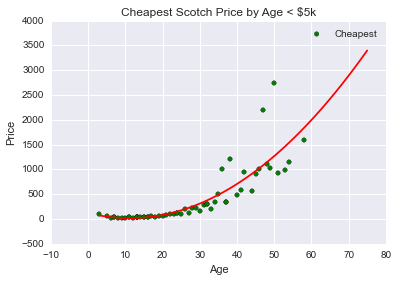
\includegraphics[scale=1]{cheapest_price_by_age} 
\caption{Cheapest whiskies by age}
\label{fig:cheapest} 
\end{figure}

One of the more interesting results from this study was that while the most expensive whiskies per age group were very noisy, the cheapest price per age fits a beautiful quadratic curve.

\begin{equation*}
\begin{split}
    \hat{y} &= 0.83003484 \cdot x^2 -18.5544543 \cdot x + 120.39902851\\
\end{split}
\end{equation*}


%%%%%%%%%%%%%%%%%%%%%%%%%%%%%%%%%%%%%%%%%%%%%%%%%
%%%%% Testing Claims
%%%%%%%%%%%%%%%%%%%%%%%%%%%%%%%%%%%%%%%%%%%%%%%%%
\subsection{Testing Claims}

\textit{K\&L Wines} sells the ubiquitous Glenlivet 12 Year Old for \$27.29. As we've seen so far, this is on the extreme low side, particularly for a 12 year old whisky. They claim, however, that it is \$37 elsewhere, implying that is the mean price of this particular whisky.\cite{KLWines}

We can easily test that claim against the alternative hypothesis that the mean price of The Glenlivet 12 Year Old is less than \$37.00. 

We pull the following eleven prices from various retailers in our database: \$36.98, \$27.99, \$29.99, \$39.99, \$27.99, \$27.99, \$29.99, \$32.95, \$34.99, \$39.99, and \$44.99. 


\begin{equation*}
\begin{split}
    H_0 &: \mu = \mu_0 \\
    H_1 &: \mu < \mu_0 \\
    n &= 11\\
    \mu_0 &= \$37.00\\
    \overline{x} &= 33.98\repeating{54}\\
    s &= 5.59237689528\\
    \alpha &= 0.05\\
    t_{10, 0.05} &= -1.812\\
\end{split}
\end{equation*}

Using our test statistic, we find
\begin{equation*}
\begin{split}
    \frac{\overline{x} - \mu_0}{\frac{\sigma}{\sqrt{n}}} &\leq -t_{10, 0.05}\\
    \frac{33.98\repeating{54} - 37.00}{\frac{5.59237689528}{\sqrt{11}}} &\leq -1.812\\
    -1.78781158232 &\leq -1.812 \XBox\\
\end{split}
\end{equation*}

We do not have enough evidence to reject their claim at the 0.05 level of significance. Their claim does not appear to be exaggerated.

I often come across "listicles" or reviews of scotch and I usually scoff at their claims of the prices of scotch. There aren't any liquor stores in my neighborhood, so the very small selection of bottles the local grocers have are extremely marked up when compared to prices claimed by various online articles. However, since we have a dataset, we can now test these claims statistically, rather than by assumption.

\textit{Thrillist}, a lifestyle and leisure website published an article entitled \textit{10 Scotches Under \$50 That You Should Be Drinking}. One claim I found extraordinary, was that a Highland Park 12 Year Old can be had for just \$46.

\begin{displayquote}
This scotch is like a solar eclipse. One just can't help but stare at the color of Highland Park; it's a deep warm amber that you can almost taste. The 12-year-old's heather-honey taste is attributed to the time its spent in ex-sherry casks—which gives this bottle some individuality and depth. All the good for \$46. \cite{Thrillist}
\end{displayquote}

I am not the only one dubious of this claim. In the comments, reader Noah Bieber says, \textit{"Highland park for \$46? Yea good luck with that..."} 

Let's test this claim, against the alternative that Highland Park 12 Year Old is actual more expensive on average than \$46.

We find the following prices in our database: \$44.99, \$44.99, \$45.99, \$46.99, \$49.98, \$49.99, \$51.95, \$52.99, \$54.0, \$59.99, \$59.99, \$59.99, and \$64.99.

Surprisingly, Highland Park 12 Year Old can be found for as low as \$44.99. If we are interpreting \textit{Thrillist's} claims as the lowest price, then they have already been proven right. But the article does not link to the particular retailers selling at this price, so we will make the assumption that the claim is for the average market value.

\begin{equation*}
\begin{split}
    H_0 &: \mu = \mu_0 \\
    H_1 &: \mu > \mu_0 \\
    \mu_0 &= \$46.00\\
    n &= 13\\
    \overline{x} &= 52.8330769231\\
    s &= 6.34787473171\\
    \alpha &= 0.05\\
    t_{12, 0.05} &= 1.782\\
\end{split}
\end{equation*}

Using our test statistic, we find
\begin{equation*}
\begin{split}
    \frac{\overline{x} - \mu_0}{\frac{\sigma}{\sqrt{n}}} &\geq -t_{12, 0.05}\\
    \frac{52.8330769231 - 46.00}{\frac{6.34787473171}{\sqrt{13}}} &\geq 1.782\\
    3.88114294258 &\geq 1.782 \checkmark\\
\end{split}
\end{equation*}

We can definitely reject the claim that on average, a Highland Park 12 Year Old can be found for \$46.00 with a $p$-value $< 0.005$. 

\pagebreak

%%%%%%%%%%%%%%%%%%%%%%%%%%%%%%%%%%%%%%%%%%%%%%%%%
%%%%% Comparing Online Retailers
%%%%%%%%%%%%%%%%%%%%%%%%%%%%%%%%%%%%%%%%%%%%%%%%%
\section{Ranking Online Retailers}

17 retailers were considered in this study. Three additional retailers were rejected because either they did not have the option of shipping out of state, or the customs import fees were too high to consider. Furthermore, UK based retailers deal primarily in 700 ml bottles, which is the standard volume for the UK, making comparisons slightly skewed. There are undoubtedly many other retailers out there, including local retailers that may have better prices, but this study gives a good feel for the competition and price spread.

\begin{figure}[htb]
\centering
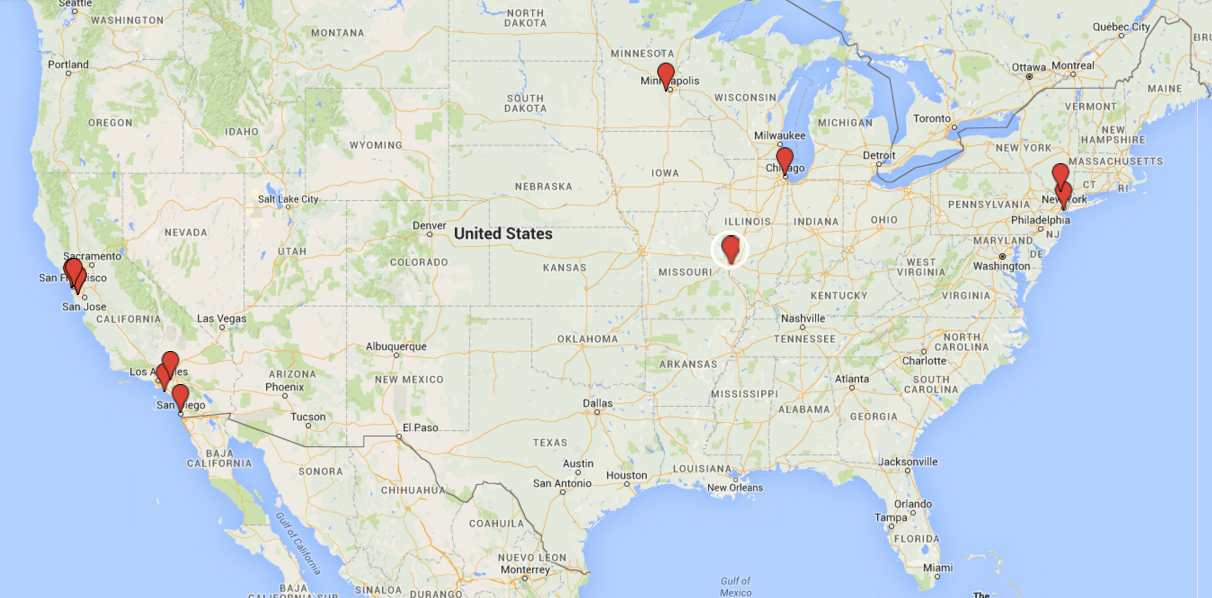
\includegraphics[scale=.3]{retailer_locations} 
\caption{Brick and mortar locations of online retailers. Caskers, Love Scotch, Pacific Online Spirits, and Ultimate Wine Shop have no brick and mortar shops.}
\label{fig:retailer_locations} 
\end{figure}

While the primary goal of this paper is to meet the requirements of MATH 8756 (Probability and Statistics II), a secondary personal goal was to find the cheapest online retailers of scotch in general. To do this, I developed an algorithm that makes use of the data and compares each online retailer with the others and gives each one an overall score. The smaller the score the better the prices when compared with the other retailers.

The algorithm uses two matrices; $\matr{P}$, the price matrix, which holds all of the prices we want to compare, and $\matr{C}$, the comparison matrix, which holds the scores of the retailers and is used to compute the final scores.

%%%%%%%%%%%%%%%%%%%%%%%%%%%% EXAMPLE MATRIX
\begin{equation*}
\begin{split}
    \matr{P} &= 
    \begin{bmatrix}[c | c c c c]
    s_{11}       & x_{12} & x_{13} & \dots & x_{1n} \\
    s_{21}       & x_{22} & x_{23} & \dots & x_{2n} \\
    \vdots       & \vdots & \vdots & \ddots & \vdots \\
    %    \hdotsfor{5} \\
    s_{m1}       & x_{m2} & x_{m3} & \dots & x_{mn}
    \end{bmatrix}\\
\end{split}
\end{equation*}

The first column of $s$ variables is the scotch ID. The other columns are for the retailers, and the $x$ variables are the prices for each retailer pertaining to the scotch ID.


%%%%%%%%%%%%%%%%%%%%%%%%%%%% EXAMPLE MATRIX
\begin{equation*}
\begin{split}
    \matr{C} &= 
    \begin{bmatrix}[c c c c c]
    x_{11} & x_{12} & x_{13} & \dots & x_{1n} \\
    x_{21} & x_{22} & x_{23} & \dots & x_{2n} \\ \vdots & \vdots & \vdots & \ddots & \vdots \\
    %    \hdotsfor{5} \\
    x_{m1} & x_{m2} & x_{m3} & \dots & x_{mn}
    \end{bmatrix}\\
\end{split}
\end{equation*}

We begin by initializing the $\matr{C}$ matrix to all zeroes,

\begin{equation*}
\begin{split}
    \matr{C} &:= 0 \cdot \matr{C}\\
\end{split}
\end{equation*}

Then, we compare each retailer with the other retailers by scotch. If one retailer does not have a price for a particular scotch, we do not compare the two. 

\pagebreak

\begin{algorithmic}
\State $j \gets 1$
\For {$j \leq$ Len($\matr{P}_0$)}
    \State $k \gets j$
    \For {$k \leq$ Len($\matr{P}_0$)}
        \State $i \gets 0$
        \For {$i \leq$ Len($\matr{P}$)}
            \State $\matr{C}_{j - 1,k - 1} \gets \matr{C}_{j - 1,k - 1} + (\matr{P}_{ij} - \matr{P}_{ik})$
            \State $\matr{C}_{k - 1,j - 1} \gets - (\matr{C}_{k - 1,j - 1} + (\matr{P}_{ij} - \matr{P}_{ik}))$
            \State $i \gets i + 1$
        \EndFor
        \State $k \gets k + 1$
    \EndFor
    \State $j \gets j + 1$
\EndFor
\end{algorithmic}

What we end up with is the hollow $N \times N$ matrix $\matr{C}$, with 

\begin{equation*}
    tr(C) = \sum_{i = 1}^N a_{ii} = 0
\end{equation*}

By summing the rows, we end up with a rank for each retailer, $r_i \in {\rm I\!R}$, such that $min(r_i)$ reflects the retailer with the lowest overall prices.

\begin{figure}[htb]
\centering
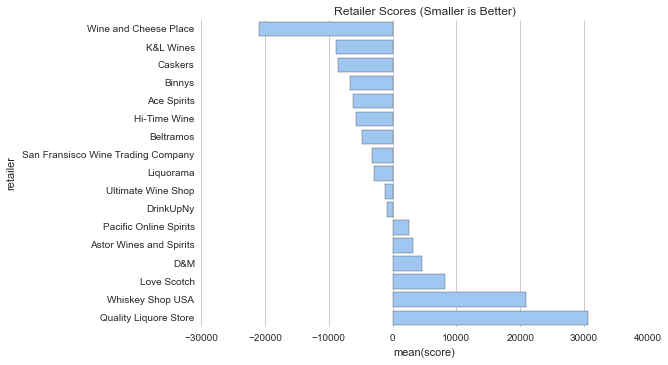
\includegraphics[scale=.5]{retailer_rankings} 
\caption{Results of retailer ranking algorithm}
\label{fig:retailer_rankings} 
\end{figure}

\pagebreak

In this case, Wine and Cheese Place has the best all around prices, and Quality Liquore Store has the worst. Price is only one factor, however, as there are several opportunities for add-on charges that were not accounted for here, including taxes, shipping, discounts for larger orders, and specials. The winner here, for instance, charges \$24.99 out of state FedEx shipping. An online-only retailer such as Caskers may end up beating them out in the all-in price. If you happen to live near St. Louis, however, selecting the in-store pickup option can save you a lot of money. The bottom line is, this covers one metric. Make sure to shop around to find the best deals.
\chapter{Future Work}

It should be clear by this point, that while age does not imply price, prices can vary wildly among retailers. This kind of information would be incredibly valuable to consumers in the form of either a web app or mobile app. The ability to scan a barcode in-store and get an instant price comparison or to type in a whisky and get a list of prices in ascending order would be very useful for consumers.

In order for this to happen, the infrastructure would need to be more sophisticated than what I did here. The data capture and cleaning methods were intended for one-time use, but for an app like this, prices would need to be updated much more frequently and in an automated fashion. 

I suggested Natural Language Processing earlier. This is because scotches don't have easy to categorize names like beer or wine. There are complications like independent bottlers, vintages, and collectible one-offs. There are cask strength versions and different cask type variations. Narrowing this down to a single SKU for each bottle becomes even more difficult when online retailers don't use a unified naming convention. 

I was unable to successfully match many bottle listings by hand, so it would be interesting to see how something like a Bayesian text classifier could do.

The findings here open the door to more research, and since this project is open source, it is free to grow.
\chapter{Conclusion}

In this paper, first and foremost, we saw that age does not imply price. But we also saw that the lower bound of price by age can be fit to a quadratic.

We also saw that prices can vary wildly by age and by retailer, but using the algorithm presented in 2.3, we have a list of places to look in order of best to worst. Of course, only the prices of the bottles were considered, not shipping, sales, minimum orders, etc. So while the algorithm doesn't exactly make a decision for you, it does make your decision easier, and could, in the future, be made to make the decision entirely.


\cleardoublepage
%\pagebreak
\phantomsection
\addcontentsline{toc}{chapter}{References}
\begin{thebibliography}{99}

\bibitem{Macallan64}The Macallan 64 Years Old in Lalique Cire Perdue,\ \url{http://us.themacallan.com/the-whisky/limited-releases/the-macallan-64-years-old-in-lalique-cire-perdue/}

\bibitem{WhiskeyDB}Whiskey Database,\ \url{http://whiskyanalysis.com/index.php/methodology-introduction/methodology-biases-and-limitations/}

\bibitem{Chivas}Whisky Advocate,\ \url{http://whiskyadvocate.com/2010/06/28/what-does-a-whiskys-age-really-mean/}

\bibitem{WhiskyDotCom}Whisky.com,\
\url{https://www.whisky.com/whisky-database/database.html}

\bibitem{WhiskyStats}Whiskeystats.net,\
\url{http://www.whiskystats.net/}

\bibitem{WhiskyAnalysis}WhiskyAnalysis.com\
\url{http://whiskyanalysis.com/}

\bibitem{WhiskyMaps}Whiskybase.com Maps,\
\url{https://www.whiskybase.com/maps}

\bibitem{Finney}D. J. Finney,\
On the distribution of a variate whose logarithm is normally distributed,\ J. Roy. Statist. Soc. Ser. B, \textbf{7} (1941), pp. 155-161

\bibitem{Shen}Wei-Hsiung Shen,\
Estimation of Parameters of a Lognormal Distribution,\ Taiwanese Journal of Mathematics,\ Vol.2, No. 2, pp. 243-250, June 1998

\bibitem{KLWines}K\&L Wines,The Glenlivet 12 Year Old\
\url{http://www.klwines.com/p/i?i=620004}

\bibitem{Thrillist}Thrillist,10 Scotches Under \$50 That You Should Be Drinking\
\url{https://www.thrillist.com/vice/best-scotch-whisky-under-50-johnnie-walker-glenlivet-laphroaig}

\bibitem{StatisticsDoneWrong}Reinhart, Alex (2015). \textit{Statistics Done Wrong}.
San Francisco:\
No Starch Press, Inc.

\bibitem{GitHub}Detweiler, Brian. MATH 8756 Final Project,\
\url{https://github.com/bdetweiler/math-8756-final-project}

\end{thebibliography}


\begin{appendices}
\chapter{Whiskies 12 Years or Older Under \$50}
\label{sec:Bargains}

\begin{center}
 \begin{tabular}{||c | c | c | c | c ||} 
 \hline
Producer & Distillery & Age & Price & Retailer\\
 \hline
 \hline
Lismore & Unknown Speyside & 15 & 39.99 & Liquorama\\
\hline
Tullibardine & Tullibardine & 14 & 39.99 & Binnys\\
\hline
Lismore & Unknown Speyside & 15 & 39.99 & Hi-Time Wine\\
\hline
Lismore & Unknown Speyside & 15 & 41.95 & Love Scotch\\
\hline
William Maxwell and Co. &  & 18 & 41.98 & Ace Spirits\\
\hline
Glenfiddich & Glenfiddich & 14 & 44.98 & Hi-Time Wine\\
\hline
Glen Moray & Glen Moray & 16 & 44.99 & Binnys\\
\hline
Glenlivet & Glenlivet & 15 & 44.99 & Hi-Time Wine\\
\hline
Tomintoul & Tomintoul & 16 & 44.99 & Ultimate Wine Shop\\
\hline
Lismore & Unknown Speyside & 15 & 44.99 & Wine and Cheese\\
\hline
William Lundie and Co. &  & 15 & 48.99 & Ace Spirits\\
\hline
Glenfiddich & Glenfiddich & 14 & 49.99 & Liquorama\\
\hline
Lismore & Unknown Speyside & 18 & 49.99 & Liquorama\\
\hline
Glenlivet & Glenlivet & 15 & 49.99 & Liquorama\\
\hline
Craigellachie & Craigellachie & 13 & 49.99 & Astor\\
\hline
Tomatin & Tomatin & 15 & 49.99 & Quality Liquore Store\\
\hline
Glenfiddich & Glenfiddich & 14 & 49.99 & Binnys\\
\hline
Tullibardine & Tullibardine & 14 & 49.99 & Binnys\\
\hline
Glenfiddich & Glenfiddich & 14 & 49.99 & Beltramos\\
\hline
Glenlivet & Glenlivet & 15 & 49.99 & Beltramos\\
\hline
Craigellachie & Craigellachie & 13 & 49.99 & Caskers\\
\hline
Tobermory & Tobermory & 15 & 49.99 & Caskers\\
\hline
Dalwhinnie & Dalwhinnie & 15 & 49.99 & K\&L Wines\\
\hline
Craigellachie & Craigellachie & 13 & 49.99 & Hi-Time Wine\\
\hline
Glenfiddich & Glenfiddich & 15 & 49.99 & Hi-Time Wine\\
\hline
Craigellachie & Craigellachie & 13 & 49.99 & Wine and Cheese\\
\hline
Glenfiddich & Glenfiddich & 15 & 49.99 & Wine and Cheese\\
[1ex]
\hline
\end{tabular}
\label{table:1}
\end{center}
\begin{center}
    Whiskies over 12 years old under \$50
\end{center}

\chapter{Whiskies over \$5,000}

\begin{center}
 \begin{tabular}{||c | c | c | c  ||} 
 \hline
Producer & Distillery & Age & Price \\
 \hline
 \hline
Signatory Vintage & Glenfarclas & 40 years old & \$5,249.99\\
Tobermory & Tobermory & 42 years old & \$5,250.0\\
Macallan & Macallan & 25 years old & \$5,299.0\\
Tobermory & Tobermory & 42 years old & \$5,499.0\\
Balvenie & Balvenie & 40 years old & \$6,069.95\\
Macallan & Macallan & 26 years old & \$6,299.0\\
Gordon \& MacPhail & Glenlivet & 61 years old & \$9,999.0\\
Gordon \& MacPhail & Linkwood & 61 years old & \$9,999.0\\
Gordon \& MacPhail & Mortlach & 63 years old & \$9,999.0\\
Gordon \& MacPhail & Strathisla & 57 years old & \$9,999.0\\
Macallan & Macallan & 68 years old & \$9,999.0\\
Bowmore & Bowmore & 38 years old & \$9,999.99\\
Macallan & Macallan & 30 years old & \$13,999.0\\
Glen Grant & Glen Grant & 50 years old & \$14,999.0\\
Glen Grant & Glen Grant & 50 years old & \$14,999.0\\
Highland Park & Highland Park & 50 years old & \$15,999.0\\
Gordon \& MacPhail & Glen Grant & 60 years old & \$16,999.0\\
Macallan & Macallan & 36 years old & \$16,999.0\\
Macallan & Macallan & 65 years old & \$17,999.0\\
Macallan & Macallan & 52 years old & \$19,000.0\\
Duncan Taylor & Macallan & 42 years old & \$19,899.99\\
Glenfarclas & Glenfarclas & 60 years old & \$19,999.99\\
Mortlach & Mortlach & 70 years old & \$20,999.99\\
Bowmore & Bowmore & 50 years old & \$21,999.0\\
Macallan & Macallan & 50 years old & \$22,499.0\\
Macallan & Macallan & 50 years old & \$22,999.99\\
Macallan & Macallan & 56 years old & \$26,999.0\\
Macallan & Macallan & 62 years old & \$27,999.99\\
Macallan & Macallan & 62 years old & \$29,500.0\\
Glenfiddich & Glenfiddich & 50 years old & \$29,999.0\\
Gordon \& MacPhail & Mortlach & 75 years old & \$31,000.0\\
Macallan & Macallan & 37 years old & \$31,748.99\\
Macallan & Macallan & 30 years old & \$31,999.99\\
Macallan & Macallan & 37 years old & \$32,374.99\\
Gordon \& MacPhail & Mortlach & 75 years old & \$34,999.0\\
Balvenie & Balvenie & 50 years old & \$43,999.0\\
\hline
\end{tabular}
\label{table:2}
\end{center}

\end{appendices}

\end{document}
